% 若编译失败,且生成 .synctex(busy) 辅助文件,可能有两个原因:
% 1. 需要插入的图片不存在:Ctrl + F 搜索 'figure' 将这些代码注释/删除掉即可
% 2. 路径/文件名含中文或空格:更改路径/文件名即可

% --------------------- 文章宏包及相关设置 --------------------- %
% >> ------------------ 文章宏包及相关设置 ------------------ << %
% 设定文章类型与编码格式
\documentclass[UTF8]{report}		

% 本文特殊宏包

% 自定义宏定义
    \def\N{\mathbb{N}}
    \def\F{\mathbb{F}}
    \def\Z{\mathbb{Z}}
    \def\Q{\mathbb{Q}}
    \def\R{\mathbb{R}}
    \def\C{\mathbb{C}}
    \def\T{\mathbb{T}}
    \def\S{\mathbb{S}}
    \def\A{\mathbb{A}}
    \def\I{\mathscr{I}}
    \def\Arg{\mathrm{Arg}}
    \def\d{\mathrm{d}}
    \def\p{\partial}


% 导入基本宏包
    \usepackage[UTF8]{ctex}     % 设置文档为中文语言
    \usepackage[colorlinks, linkcolor=blue, anchorcolor=blue, citecolor=blue, urlcolor=blue]{hyperref}  % 宏包:自动生成超链接 (此宏包与标题中的数学环境冲突)
    % \usepackage{docmute}    % 宏包:子文件导入时自动去除导言区,用于主/子文件的写作方式,\include{./51单片机笔记}即可。注:启用此宏包会导致.tex文件capacity受限。
    \usepackage{amsmath}    % 宏包:数学公式
    \usepackage{mathrsfs}   % 宏包:提供更多数学符号
    \usepackage{amssymb}    % 宏包:提供更多数学符号
    \usepackage{pifont}     % 宏包:提供了特殊符号和字体
    \usepackage{extarrows}  % 宏包:更多箭头符号
    \usepackage{multicol}   % 宏包:支持多栏 


% 文章页面margin设置
    \usepackage[a4paper]{geometry}
        \geometry{top=1in}  % 1 inch= 2.46 cm, 0.75 inch = 1.85 cm
        \geometry{bottom=1in}
        \geometry{left=0.75in}
        \geometry{right=0.75in}   % 设置上下左右页边距
        \geometry{marginparwidth=1.75cm}    % 设置边注距离(注释、标记等)

% 配置数学环境
    \usepackage{amsthm} % 宏包:数学环境配置
    % theorem-line 环境自定义
        \newtheoremstyle{MyLineTheoremStyle}% <name>
            {11pt}% <space above>
            {11pt}% <space below>
            {}% <body font> 使用默认正文字体
            {}% <indent amount>
            {\bfseries}% <theorem head font> 设置标题项为加粗
            {:}% <punctuation after theorem head>
            {.5em}% <space after theorem head>
            {\textbf{#1}\thmnumber{#2}\ \ (\,\textbf{#3}\,)}% 设置标题内容顺序
        \theoremstyle{MyLineTheoremStyle} % 应用自定义的定理样式
        \newtheorem{LineTheorem}{Theorem.\,}
    % theorem-block 环境自定义
        \newtheoremstyle{MyBlockTheoremStyle}% <name>
            {11pt}% <space above>
            {11pt}% <space below>
            {}% <body font> 使用默认正文字体
            {}% <indent amount>
            {\bfseries}% <theorem head font> 设置标题项为加粗
            {:\\ \indent}% <punctuation after theorem head>
            {.5em}% <space after theorem head>
            {\textbf{#1}\thmnumber{#2}\ \ (\,\textbf{#3}\,)}% 设置标题内容顺序
        \theoremstyle{MyBlockTheoremStyle} % 应用自定义的定理样式
        \newtheorem{BlockTheorem}[LineTheorem]{Theorem.\,} % 使用 LineTheorem 的计数器
    % definition 环境自定义
        \newtheoremstyle{MySubsubsectionStyle}% <name>
            {11pt}% <space above>
            {11pt}% <space below>
            {}% <body font> 使用默认正文字体
            {}% <indent amount>
            {\bfseries}% <theorem head font> 设置标题项为加粗
            {:\\ \indent}% <punctuation after theorem head>
            {0pt}% <space after theorem head>
            {\textbf{#3}}% 设置标题内容顺序
        \theoremstyle{MySubsubsectionStyle} % 应用自定义的定理样式
        \newtheorem{definition}{}

%宏包:有色文本框(proof环境)及其设置
    \usepackage[dvipsnames,svgnames]{xcolor}    %设置插入的文本框颜色
    \usepackage[strict]{changepage}     % 提供一个 adjustwidth 环境
    \usepackage{framed}     % 实现方框效果
        \definecolor{graybox_color}{rgb}{0.95,0.95,0.96} % 文本框颜色。修改此行中的 rgb 数值即可改变方框纹颜色,具体颜色的rgb数值可以在网站https://colordrop.io/ 中获得。(截止目前的尝试还没有成功过,感觉单位不一样)(找到喜欢的颜色,点击下方的小眼睛,找到rgb值,复制修改即可)
        \newenvironment{graybox}{%
        \def\FrameCommand{%
        \hspace{1pt}%
        {\color{gray}\small \vrule width 2pt}%
        {\color{graybox_color}\vrule width 4pt}%
        \colorbox{graybox_color}%
        }%
        \MakeFramed{\advance\hsize-\width\FrameRestore}%
        \noindent\hspace{-4.55pt}% disable indenting first paragraph
        \begin{adjustwidth}{}{7pt}%
        \vspace{2pt}\vspace{2pt}%
        }
        {%
        \vspace{2pt}\end{adjustwidth}\endMakeFramed%
        }

% 外源代码插入设置
    % matlab 代码插入设置
    \usepackage{matlab-prettifier}
        \lstset{
            style=Matlab-editor,  % 继承matlab代码颜色等
        }
    \usepackage[most]{tcolorbox} % 引入tcolorbox包 
    \usepackage{listings} % 引入listings包
        \tcbuselibrary{listings, skins, breakable}
        \lstdefinestyle{matlabstyle}{
            language=Matlab,
            basicstyle=\small,
            breakatwhitespace=false,
            breaklines=true,
            captionpos=b,
            keepspaces=true,
            numbers=left,
            numbersep=15pt,
            showspaces=false,
            showstringspaces=false,
            showtabs=false,
            tabsize=2
        }
        \newtcblisting{matlablisting}{
            arc=0pt,
            top=0pt,
            bottom=0pt,
            left=1mm,
            listing only,
            listing style=matlabstyle,
            breakable,
            colback=white   % 选一个合适的颜色
        }

% table 支持
    \usepackage{booktabs}   % 宏包:三线表
    \usepackage{tabularray} % 宏包:表格排版
    \usepackage{longtable}  % 宏包:长表格

% figure 设置
    \usepackage{graphicx}  % 支持 jpg, png, eps, pdf 图片 
    \usepackage{svg}       % 支持 svg 图片
        \svgsetup{
            % 指向 inkscape.exe 的路径
            inkscapeexe = D:/aa_my_apps_main/Inkscape/bin/inkscape.exe, 
            % 一定程度上修复导入后图片文字溢出几何图形的问题
            inkscapelatex = false                 
        }

% 图表进阶设置
    \usepackage{caption}    % 图注、表注
        \captionsetup[figure]{name=图}  
        \captionsetup[table]{name=表}
        \captionsetup{labelfont=bf, font=small}
    \usepackage{float}     % 图表位置浮动设置 

% 圆圈序号自定义
    \newcommand*\circled[1]{\tikz[baseline=(char.base)]{\node[shape=circle,draw,inner sep=0.8pt, line width = 0.03em] (char) {\small \bfseries #1};}}   % TikZ solution

% 列表设置
    \usepackage{enumitem}   % 宏包:列表环境设置
        \setlist[enumerate]{itemsep=0pt, parsep=0pt, topsep=0pt, partopsep=0pt, leftmargin=3.5em} 
        \setlist[itemize]{itemsep=0pt, parsep=0pt, topsep=0pt, partopsep=0pt, leftmargin=3.5em}
        \newlist{circledenum}{enumerate}{1} % 创建一个新的枚举环境  
        \setlist[circledenum,1]{  
            label=\protect\circled{\arabic*}, % 使用 \arabic* 来获取当前枚举计数器的值,并用 \circled 包装它  
            ref=\arabic*, % 如果需要引用列表项,这将决定引用格式(这里仍然使用数字)
            itemsep=0pt, parsep=0pt, topsep=0pt, partopsep=0pt, leftmargin=3.5em
        }  

% 其它设置
    % 脚注设置
        \renewcommand\thefootnote{\ding{\numexpr171+\value{footnote}}}
    % 参考文献引用设置
        \bibliographystyle{unsrt}   % 设置参考文献引用格式为unsrt
        \newcommand{\upcite}[1]{\textsuperscript{\cite{#1}}}     % 自定义上角标式引用
    % 文章序言设置
        \newcommand{\cnabstractname}{序言}
        \newenvironment{cnabstract}{%
            \par\Large
            \noindent\mbox{}\hfill{\bfseries \cnabstractname}\hfill\mbox{}\par
            \vskip 2.5ex
            }{\par\vskip 2.5ex}

% 文章默认字体设置
\usepackage{fontspec}   % 宏包:字体设置
    \setmainfont{SimSun}    % 设置中文字体为宋体字体
    \setCJKmainfont[AutoFakeBold=3]{SimSun} % 设置加粗字体为 SimSun 族,AutoFakeBold 可以调整字体粗细
    \setmainfont{Times New Roman} % 设置英文字体为Times New Roman

% 各级标题自定义设置
\usepackage{titlesec}   
\titleformat{\chapter}[hang]{\normalfont\huge\bfseries\centering}{第\,\thechapter\,章}{20pt}{}
\titlespacing*{\chapter}{0pt}{-20pt}{20pt} % 控制上方空白的大小
% section标题自定义设置 
\titleformat{\section}[hang]{\normalfont\Large\bfseries}{§\,\thesection\,}{8pt}{}
% subsubsection标题自定义设置
%\titleformat{\subsubsection}[hang]{\normalfont\bfseries}{}{8pt}{}

% --------------------- 文章宏包及相关设置 --------------------- %
% >> ------------------ 文章宏包及相关设置 ------------------ << %

% ------------------------ 文章信息区 ------------------------ %
% ------------------------ 文章信息区 ------------------------ %
% 页眉页脚设置
    \usepackage{fancyhdr}   %宏包:页眉页脚设置
        \pagestyle{fancy}
        \fancyhf{}
        \cfoot{\thepage}
        \renewcommand\headrulewidth{1pt}
        \renewcommand\footrulewidth{0pt}
        \lhead{2024.8-2025.1}
        \chead{Notes of Mathematical Physics Methods}     
        \rhead{dingyi233@mails.ucas.ac.cn}
%文档信息设置
\title{数学物理方法笔记\\Notes of Mathematical Physics Methods}
\author{丁毅\\ \footnotesize 中国科学院大学,北京 100049\\ Yi Ding \\ \footnotesize University of Chinese Academy of Sciences, Beijing 100049, China}
\date{\footnotesize 2024.8 -- 2025.1}
% ------------------------ 文章信息区 ------------------------ %
% ------------------------ 文章信息区 ------------------------ %

% 开始编辑文章

\begin{document} 
\zihao{5}             % 设置全文字号大小, -4 为小四, 5 为五号

% ------------------------ 封面序言与目录 ------------------------ %
% >> --------------------- 封面序言与目录 --------------------- << %
% 封面
    \maketitle\newpage  
    \pagenumbering{Roman} % 页码为大写罗马数字
    \thispagestyle{fancy}   % 显示页码、页眉等

% 序言
    \begin{cnabstract}\normalsize 
        本文为笔者本科时的数学物理方法笔记笔记,总结了数学物理方法中的主要知识,也有适当的拓展延伸。同时,对一些晦涩的概念或公式,给出了笔者的个人理解,以帮助阅读。\par
        由于个人精力及知识水平有限,书中难免有不妥、错误之处,望不吝指正,在此感谢。我的邮箱是 dingyi233@mails.ucas.ac.cn 。
    \end{cnabstract}
    \addcontentsline{toc}{chapter}{序言} % 手动添加为目录

% 目录
    \setcounter{tocdepth}{2}                % 目录深度(为1时显示到section)
    \tableofcontents                        % 目录页
    \addcontentsline{toc}{chapter}{目录}    % 手动添加此页为目录
    \thispagestyle{fancy}                   % 显示页码、页眉等 

% 收尾工作
    \newpage    
    \pagenumbering{arabic} 


% >> --------------------- 封面序言与目录 --------------------- << %
% ------------------------ 封面序言与目录 ------------------------ %




\chapter{复数与复数运算}\thispagestyle{fancy} 
\section{预备知识}


\begin{definition}[复数定义]
    一个有序实数对 $(x,y)$ 称为复数如果其满足如下运算:
\begin{gather}
    \begin{aligned}
        &\text{加法}&&(x_1,y_1)+(x_2,y_2)=(x_1+x_2,y_1+y_2)\\
        &\text{乘法}&&(x_1,y_1)(x_2,y_2)=(x_1x_2-y_1y_2,x_1y_2+y_1x_2)
    \end{aligned}
\end{gather}
记作 $z = x + iy$,其中 $x = \R z$,$y = \I z$,$i^2 = 1$。

\end{definition}


\begin{definition}[相关概念] 
    下面是一些相关概念:
\begin{circledenum}
    \item 复数的三种表示:$z = x + iy = r(\cos \theta + i\sin \theta) =  re^{i\theta} = e^{\ln r + i\theta}$
    \item 模:$|z| = r =\sqrt{x^2+y^2}$
    \item 幅角:$\arg z = \theta \in (-\pi, \pi]$称为幅角主值,$\Arg z = \theta + 2k\pi$称为幅角补值,$k\in\Z$。
    \item 0 与 $\infty$:是两个特殊的复数,分别表示复平面中模为 0 和无穷大而幅角任意的“一个点”。在复平面的球表示中,$0$ 对应南极,$\infty$ 对应北极。
    \item 扩充复平面:称包含无穷远点 $\infty$ 的复平面 $\overline{\C} = \C \cup \{\infty\}$为扩充复平面。
    \item 共轭复数:$ z = x + iy, z^* = x - iy$
    \item 复数除法:设$z_1 = x_1 + iy_1, z_2 = x_2 + iy_2$,则:
    \begin{equation}
    \frac{z_1}{z_2}= \frac{x_1+\mathrm{i}y_1}{x_2+\mathrm{i}y_2}=\frac{(x_1+\mathrm{i}y_1)(x_2-\mathrm{i}y_2)}{(x_2+\mathrm{i}y_2)(x_2-\mathrm{i}y_2)} = \frac{1}{| z_2 |^2}\left[ (x_1x_2+y_1y_2) + \mathrm{i}(y_1x_2-x_1y_2) \right]
    \end{equation}
    用棣莫弗定理更易理解复数除法:设 $z_1 = r_1e^{i\theta_1}, z_2 = r_2e^{i\theta_2}$,则: 
    \begin{equation}
    \frac{z_1}{z_2} = \frac{r_1}{r_2}e^{i(\theta_1-\theta_2)}
    \end{equation}
    \item 复数乘法:$z_1z_2 = r_1r_2e^{i(\theta_1+\theta_2)}$
\end{circledenum}



\end{definition}


\section{复数序列}

\begin{definition}[相关概念]
    一个复数序列 $\{z_n\}$ 完全等价于两个实数序列 $\{x_n\}$ 和$\{y_n\}$
    \begin{circledenum}
        \item 聚点:给点复序列 $\{z_n\}$,若存在 $z \in \C$,使 $\forall\ \varepsilon >0$,恒有无穷多个$n$ 使得 $| z_n - z | < \varepsilon$则称$z$ 为序列$\{z_n\}$ 的一个聚点。
        {\par\color{gray}\small
        例如序列 $\{(-1)^{n+1}\frac n{n+1}\mid n \in \mathbb{N}_+\} =  \{\frac12,-\frac23,\frac34,-\frac45,\frac56,-\frac67,\cdots,(-1)^{n+1}\frac n{n+1},\cdots \}$ 有两个聚点 $1,-1$.
        \par}
        \item 有界 / 无界序列:序列 $\{z_n\}$ 称为有界的如果 $\exists\ M>0 \ \ \text{s.t.}\ \ | z_n | < M,\ \forall\ n \in \mathbb{N}_+$,否则称为无界的。
        \item 极限:称序列$\{z_n\}$收敛于$z \in \C$ 如果 $ \forall\ \varepsilon > 0,\ \exists\ N>0 \ \ \text{s.t.}\ \ | z - z_n | < \varepsilon, \forall\ n > N$ ,记作 $\displaystyle \lim_{n \rightarrow \infty} z_n = z $,否则称为发散序列。
        极限的必要条件是唯一聚点,无界序列不可能收敛
    \end{circledenum}
\end{definition}

\begin{LineTheorem}[Bolzano - Weierstrass 定理]\label{Bolzano - Weierstrass 定理}
任意有界序列至少有一个聚点。
\footnote{
    Theorem.\ref{Bolzano - Weierstrass 定理} 告诉我们有界序列必有聚点,事实上,在扩充复数域 $\overline{\C}$ 中,这对无界序列也成立($\infty$ 必为聚点),也即任意序列都必有聚点。}
\end{LineTheorem}

\begin{LineTheorem}[Cauchy判别法]\label{Cauchy判别法}
序列收敛的等价条件是:$\forall\ \varepsilon > 0, \exists\ N = N(\varepsilon) \ \ \text{s.t.}\ \ | z_{N+p} - z_N | < \varepsilon, \forall\ p \in \mathbb{N}_+$。
\end{LineTheorem}

\section{复变函数}


\begin{definition}[相关概念]
如下:
\begin{circledenum}
\item 点集:复平面内点的集合
\item 区域:复点集称为区域如果全部由内点组成,且具有连通性 
\footnote{连通性:集合中任意两点都可以用一条折线连接起来,且折线上的点全部属于此点集}
\item 单连通 / 多联通区域:区域称为单连通的如果在其内作任何简单闭合围道(自身不相交的闭合曲线),围道内的点都属于该区域,否则称为多联通区域(也称复联通区域)
{\par\color{gray}\small
例如,图 \ref{(a) (b) 构成区域,(c) 不构成区域} 中的 (a) 区域就属于单连通区域,而图 \ref{(a) (b) 构成区域,(c) 不构成区域} 中的(b)区域则为多连通区域.
\par}
\item 边界:区域$G$ 的全体边界点构成其边界,记为 $\p G$
\item 边界方向:沿着区域的边界前进,区域恒保持在边界的左侧,则此走向称为边界的正向 
\end{circledenum}

\begin{figure}[H]\centering
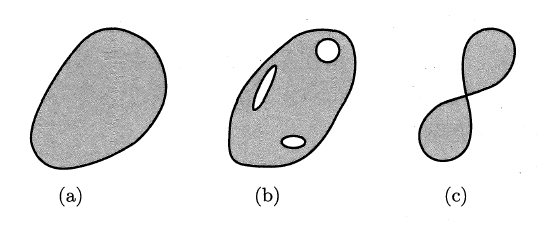
\includegraphics[width=0.45\textwidth]{assets/4d651e08624250e2b6a287f557fe1cf8.png}
\caption{\textbf{(a) (b) 构成区域,(c) 不构成区域}}\label{(a) (b) 构成区域,(c) 不构成区域}
\end{figure}
\end{definition}


\begin{definition}[复变函数]
复变函数 $f$ 是复数域子域 $G \subseteq \C$ 到复数域的映射,记作 $f:\ z \longmapsto \C$,或者 $f(z) = w,\ z \in G$。区域 $G$ 称为函数$f$  的定义域。事实上,复变函数等价于两个实变函数的有序组合。特别地,多值函数允许一个自变量对应多个函数值,我们在第二章会讨论。

\end{definition}

\section{无穷远点}

\begin{definition}[Riemann 球面]
如 图 \ref{Riemann 球面(复数球面)} ,过扩充的复平面$\overline{\C}$中的原点$(0,0)$作直径为 1 的球面,使之与$\overline{\C}$相切,切点称为南极 S,南极直径另一端称为北极 N。$\forall\ z \in \overline{\C}$,将它和复数球面的北极 N 相连,连线和球面有且仅有一个交点,因此存在一一对应关系。容易理解,$0$ 对应南极 S 而 $\infty$ 对应北极 N。

\begin{figure}[H]\centering
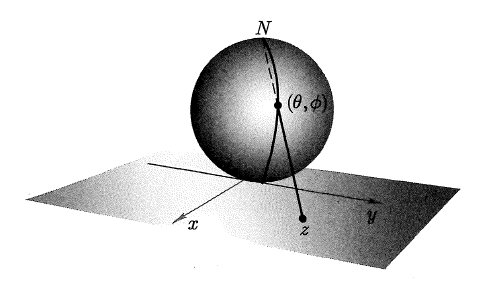
\includegraphics[width=0.40\textwidth]{assets/79ee2f440c28e683147e653d153efc72.png}
\caption{\textbf{Riemann 球面(复数球面)}}\label{Riemann 球面(复数球面)}
\end{figure}
\end{definition}

\chapter{解析函数}

\section{复变函数的极限和连续}



\begin{definition}[极限]
设复变函数 $f(z)$ 在 $z_0$ 的空心邻域 $U^\circ_{\delta}(z_0)$ 中有定义
\footnote{$z_0$ 的空心邻域是指以 $z_0$ 为圆心的环域 $0 < | z - z_0 | < \varepsilon$},
若 $\exists\ A \in \C $ 满足 $ \forall\ \varepsilon > 0,\ \exists\ \delta = \delta(\varepsilon)>0 \ \ \text{s.t.}\ \ | f(z) - A |<\varphi,\ \forall\ 0<| z - z_0 |<\delta $,则称 $z \to z_0$ 时 $f(z)$ 存在极限 $A$,记作:
\begin{equation}
\lim_{z \to z_0}f(z) = A
\end{equation} 
并且,设 $f(z) = u(z) + iv(z)$,$u,v$ 是 $\C$ 到 $\R$ 的函数,可以证明:
\begin{equation}
\lim_{z \to z_0}f(z) = \lim_{z \to z_0}u(z) + \mathrm{i}  \lim_{z \to z_0}v(z)
\end{equation} 
\end{definition}


\begin{definition}[连续]
设复变函数 $f(z)$ 在 $z_0$ 的邻域 $U_{\delta}(z_0)$ 中有定义,且 $ \lim_{z\to z_0}f(z) = f(z_0)$,则称 $f(z)$ 在 $z_0$ 处连续。

在有界必域 $\overline{G}$ 中连续的函数 $f(z)$ 具有两个重要性质:
\begin{circledenum}[leftmargin=4em]
\item  $ | f(z) | $ 在 $\overline{G}$ 中有界,并且上下界可取到
\item $f(x)$ 在 $\overline{G}$ 中一致连续,即 $| f(z_1) - f(z_2) | < \varepsilon, \forall\ | z_1 - z_2 | < \delta $
\end{circledenum}
\end{definition}


\section{可导与可微}


\begin{definition}[可导]
单值复变函数 $f(z)$ 在 $z_0$ 处可导如果 $\lim\frac{f(z + \Delta z) - f(z)}{\Delta z} = C \in \R$ 
\footnote{这要求 $\Delta z$ 以任意方式趋于零,此极限都存在,类似二元函数的导数。}
,记为 $f'(z)$。

容易证明,高等数学中的各种求导公式都可以直接搬用到复变函数。

Cauchy-Riemann 条件是函数可导的必要条件:
\begin{equation}
(\frac{\partial f }{\partial x }) = \Re (\frac{\partial f }{\partial y }) \ ,\ \ \Im (\frac{\partial f }{\partial x }) = -\Im (\frac{\partial f }{\partial y })
\end{equation}
\end{definition}


\begin{definition}[可微]
若存在 $A = A(z) \in \C \ \ \text{s.t.}\ \ \Delta f(z) = A(z) \cdot \Delta z + O(\Delta z)$,则称 $f(z)$ 在 $z_0$ 处可微,记作 $\mathrm{d} f = A \mathrm{d}z$.

和实数一样,$\mathrm{d} f = f'(z) \mathrm{d}z$,并且 可微 $\Longrightarrow$ 可导 $\Longrightarrow$ 连续。
\end{definition}

\section{解析函数}


函数 $f$ 称为 $G$ 上的解析函数如果 $f$ 在区域 $G$ 内每一点都可导,又称为 $f$ 在 $G$ 上解析。

在 $G$ 内解析的函数必满足 Cauchy-Riemann 方程,因此只要知道其中之一,例如 $f(x,y) = u(x,y) + iv(x,y)$ 的实部 $u(z)$,就可以唯一地确定其虚部(可加减实常数),这是因为:
\begin{gather}
\mathrm{d} v = \frac{\partial v }{\partial x }\mathrm{d}x + \frac{\partial v }{\partial y } \mathrm{d}y = - \frac{\partial u}{\partial y } \mathrm{d}x + \frac{\partial u}{\partial x } \mathrm{d}y \\ \Longrightarrow
v(x,y) = \int \left( - \frac{\partial u}{\partial y } \mathrm{d}x + \frac{\partial u}{\partial x } \mathrm{d}y  \right)
\end{gather}

为求此原函数,设 $v(x,y) = g_1(x,y) + g_2(y)$,则:
\begin{gather}
\frac{\partial v }{\partial x} = \frac{\partial g_1 }{\partial x } 
\Longrightarrow 
g_1(x,y) = \int \frac{\partial v }{\partial x } \mathrm{d} x = \int (- \frac{\partial u }{\partial y }) \mathrm{d}x
\\ 
\frac{\partial v }{\partial y } = \frac{\partial g_1 }{\partial y } + \frac{\partial g_2 }{\partial y } \Longrightarrow 
g_2(y) = \int (\frac{\partial v }{\partial y } - \frac{\partial g_1 }{\partial y }) \mathrm{d}y = \int (\frac{\partial u }{\partial x } - \frac{\partial g_1 }{\partial y }) \mathrm{d}y 
\end{gather}
最后相加即得 $v(x,y)$.

解析函数实部与虚部之间的这种依赖关系,还可以形象地表现出来。在 $x-y$ 平面中,分别作出 $u(x,y)$ 和 $v(x,y)$ 的等高线图,在任意一点 $(x,y)$,由 Cauchy-Reimann 方程,两者方向矢量的内积为零:
\begin{equation}
\begin{bmatrix}
    \frac{\partial u }{\partial y } & - \frac{\partial u }{\partial x }
\end{bmatrix}
\cdot 
\begin{bmatrix}
    \frac{\partial v }{\partial y } \\  -\frac{\partial v }{\partial x }
\end{bmatrix}
= \frac{\partial u }{\partial y }\frac{\partial v }{\partial y } + \frac{\partial u }{\partial x } \frac{\partial v }{\partial x } = 0
\end{equation}
因此两者的等高线图处处正交(表现为曲线处处正交)。
% {\par\color{gray}\small
% 例如 $f(z) = z^2$,则:
% \begin{gather*}
%     f(z) 
%     = \frac{1}{z^2}
%     = \frac{1}{(x^2-y^2) + (2xy) \mathrm{i} } 
%     = \frac{x^2-y^2}{(x^2 + y^2)^2} + \frac{-2xy}{(x^2 +y^2)^2}  % \mathrm{i} \\ 
%     \Longrightarrow u(x,y) = \frac{x^2-y^2}{(x^2 + y^2)^2} ,\ v(x,% y) = \frac{-2xy}{(x^2 +y^2)^2}
% \end{gather*}
% 它们的等高线图如图 ;
% \par}

{\par\color{gray}\small
例如 $f(z) = z^2$,则:
\begin{gather*}
    f(z) 
    = z^2
    = (x^2-y^2) + (2xy) \mathrm{i} 
    \Longrightarrow u(x,y) = x^2-y^2 ,\ v(x,y) = 2xy
\end{gather*}
它们的等高线图如图 \ref{解析函数 $f(z) = z^2$ 实虚部示意图} 所示:
\begin{figure}[H]\centering
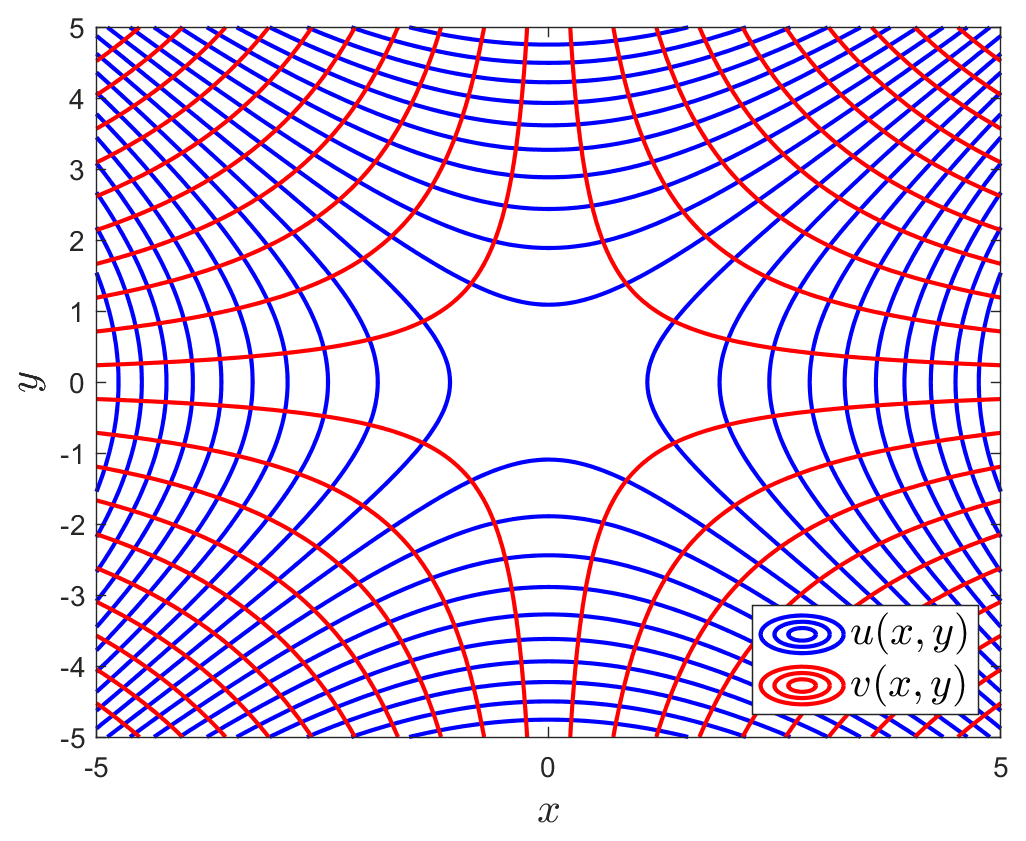
\includegraphics[width=0.45\textwidth]{assets/2024-08-28_10-23-23.png}
\caption{\textbf{解析函数 $f(z) = z^2$ 实虚部示意图}}\label{解析函数 $f(z) = z^2$ 实虚部示意图}
\end{figure}
\par}

之后我们会证明,解析函数的实部 $u(x,y)$ 和虚部 $v(x,y)$ 的二阶偏导一定存在且连续,并且满足二维 Laplace 方程,这表明解析函数的实部和虚部构成一对共轭调和函数
\footnote{共轭是因为满足 Cauchy-Riemann 方程}
。
\begin{equation}
    \Delta u = \Delta v = 0 \Longleftrightarrow
    \frac{\partial^{2}u}{\partial x^{2}}+\frac{\partial^{2}u}{\partial y^{2}}=0 \quad\frac{\partial^{2}v}{\partial x^{2}}+\frac{\partial^{2}v}{\partial y^{2}}=0
\end{equation}

函数的解析性总是和给点区域联系在一起,有时也称函数在 $z_0$ 点解析,也即在邻域 $U_{\delta}(z_0)$ 内解析。讨论解析函数的各种特殊性质,就是复变函数论的中心课题。

\section{初等函数}

一些实初等函数推广到复数域时会有比较的特殊性质,下面进行讨论。

\begin{definition}[幂函数 $z^n$]
当 $n \in \N$ 时,$z^n$ 在 $\C$ 内解析,并且当 $n \in \N^*$时,$z^n$ 在 $\infty$ 不解析;当 $n \in -\N^*$ 时,$z^n$ 在 $z=0$ 不解析,在 $\overline{\C}\setminus \{0\}$ 内解析。
\end{definition}


\begin{definition}[指数函数 $e^z$]
复指数函数在 $\C$ 内解析,但在 $\infty$ 无意义,因为极限 $\lim_{z \to \infty}e^z$ 不存在
\begin{equation}
e^z = e^{x + \mathrm{i} y} = e^x(\cos y + \mathrm{i} \sin y)
\end{equation}
\end{definition}


\begin{definition}[三角函数 $\sin z,\ \cos z,\ ...$]
复三角函数是用复指数函数定义的,如下:
\begin{equation}
    \sin z=\frac{\mathrm{e}^{\mathrm{i}z}-\mathrm{e}^{-\mathrm{i}z}}{2\mathrm{i}},\quad\cos z=\frac{\mathrm{e}^{\mathrm{i}z}+\mathrm{e}^{-\mathrm{i}z}}{2}
\end{equation}
$\sin z,\ \cos z$ 在 $\C$ 内解析,唯一奇点是 $z = \infty$。可以证明,实三角函数的各种恒等式对复三角函数仍成立。
\end{definition}


\begin{definition}[双曲函数 $\sinh z,\ \cosh z,\ ...$]
双曲函数也是通过复指数函数来定义的,如下
\begin{gather}
    \sinh z=\frac{\mathrm{e}^{z}-\mathrm{e}^{-z}}{2},\cosh z=\frac{\mathrm{e}^{z}+\mathrm{e}^{-z}}{2},\quad\tanh z=\frac{\sinh z}{\cosh z},\\\coth z=\frac{\cosh z}{\sinh z},\quad\mathrm{sech}z=\frac{1}{\cosh z},\quad\cosh z=\frac{1}{\sinh z}
\end{gather}
由定义可知,双曲函数和三角函数能够互化:
\begin{equation}
    \sinh z=-\mathrm{i}\sin\mathrm{i}z,\quad\cosh z=\cos\mathrm{i}z,\quad\tanh z=-\mathrm{i}\tan\mathrm{i}z.
\end{equation}
另外注意导数公式:
\begin{equation}
    (\sinh z)'=\cosh z,\quad(\cosh z)'=\sinh z,\quad(\tanh z)'=\mathrm{sech}^2z
\end{equation}
其它结论:
\begin{gather}
    \cosh^{2}z-\sinh^{2}z=1, \quad1-\tanh^{2}z=\mathrm{sech}^{2}z \\ 
    \sinh\left(z_{1}\pm z_{2}\right)=\sinh z_{1}\cosh z_{2}\pm\cosh z_{1}\sinh z_{2}\\
    \cosh\left(z_{1}\pm z_{2}\right)=\cosh z_{1}\cosh z_{2}\pm\sinh z_{1}\sinh z_{2}
\end{gather}
\end{definition}

\section{解析函数的保角性(略)}
\section{多值函数}

\begin{definition}[多值函数的概念]
$f$ 称为区域 $G \subseteq \C$ 上的多值函数如果 $\forall\ z \in G$ 存在多个 $w \in \C$ 使得 $f(z) = w_1 = w_2 = \cdots $。许多函数的逆运算都是多值函数。
\end{definition}

\begin{definition}[开方]
考虑 $z-a$ 的开方 $w =\sqrt{z-a}$,设 $w = \rho_1 e^{\alpha}$ 而 $z-a = \rho_2e^{\theta}$,代入解得:
\begin{gather}
     w = \sqrt{| z-a |} e^{\frac{\theta}{2} + n\pi}, \quad n \in \Z \\ \Longleftrightarrow 
     | w | = \sqrt{| z-a |},\quad \arg w = \frac{1}{2} \arg (z-a)
\end{gather}
$\omega $ 的多值性来源于 $z-a$ 幅角的多样性,我们把这样量称为\textbf{宗量}\footnote{宗量通常不同于自变量.例如,多值函数 $\sqrt{z-a}$ 的宗量就是 $z-a$,多值函数号 $\sqrt[3]{(z - a)(z - b)}$ 的宗量就是$(z-a)(z-b)$。当然,也有宗量就是自变量的情形.例如多值函数 $\sqrt{z}$ 的宗量就是自变量 $z$。}(而不是自变量)。

为了进一步揭示多值函数 $w = \sqrt{z-a}$ 的性质,我们讨论“还原”与“不还原”。在 $z$ 复平面上依次画两个圆,如图 \ref{沿闭合曲线一周回到原处时} 左侧,第一个圆在点 $a$ 外,第二个圆包含了点 $a$。

对第一种情况,$z$ 沿路径 $C_1$ 逆时针旋转一圈后,由于 $a$ 在圆外,因此旋转前后的 $\arg (z-a)$ 不变,$\arg w = \frac{1}{2} \arg (z-a)$ 也不变,从而使得旋转前后 $w$ 也不变,称为 $w$ 值“还原”。对第二种情况,$z$ 沿路径 $C_2$ 逆时针旋转一圈后,由于 $a$ 在圆内,$\arg (z-a)$ 增加了 $2\pi$ 但 $\arg w = \frac{1}{2} \arg (z-a)$ 使得 $\arg w$ 仅增加 $\pi$,从而使得旋转前后 $w$ 未回到原点,称为 $w$ 值“不还原”。

因此,点 $a$ 对多值函数 $w =\sqrt{z-a}$ 有特殊意义,它是否位于简单闭合路径内就决定了当 $z$ 沿这个路径行进一周回到原处时,相应的 $w$ 值是否能还原。


\begin{figure}[H]\centering
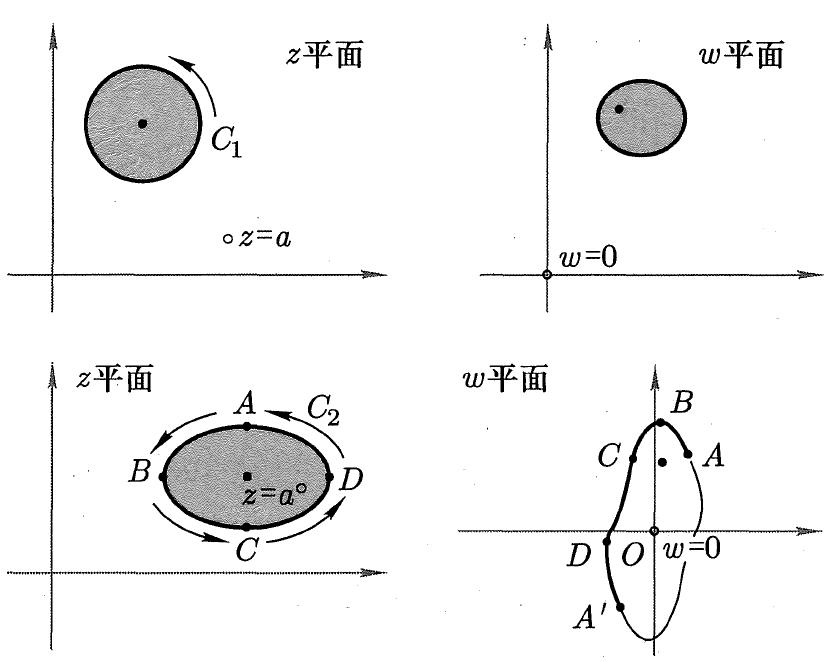
\includegraphics[width=0.55\textwidth]{assets/image (43).jpg}
\caption{\textbf{$z$ 沿闭合曲线一周回到原处时,$w = \sqrt{z-a}$ 值的不同变化}}\label{沿闭合曲线一周回到原处时}
\end{figure}

\end{definition}












































































































































































































\nocite{*}
\bibliography{re}
\thispagestyle{fancy} 
\addcontentsline{toc}{chapter}{参考文献}
\end{document}

% VScode 常用快捷键:

% F2:                       变量重命名
% Ctrl + Enter:             行中换行
% Alt + up/down:            上下移行
% 鼠标中键 + 移动:           快速多光标
% Shift + Alt + up/down:    上下复制
% Ctrl + left/right:        左右跳单词
% Ctrl + Backspace/Delete:  左右删单词    
% Shift + Delete:           删除此行
% Ctrl + J:                 打开 VScode 下栏(输出栏)
% Ctrl + B:                 打开 VScode 左栏(目录栏)
% Ctrl + `:                 打开 VScode 终端栏
% Ctrl + 0:                 定位文件
% Ctrl + Tab:               切换已打开的文件(切标签)
% Ctrl + Shift + P:         打开全局命令(设置)

% Latex 常用快捷键

% Ctrl + Alt + J:           由代码定位到PDF
% 


% Git提交规范:
% update: Linear Algebra 2 notes
% add: Linear Algebra 2 notes
% import: Linear Algebra 2 notes
% delete: Linear Algebra 2 notes